%!TEX root=./paper.tex
\section{Experiments}\label{sec:experiments}
n this section, we present the experimental results of our model, detailing the parameters necessary to replicate these outcomes. Additionally, we provide a description of the baseline models used for comparison, along with their respective parameters.

\subsection{Dataset Description}

We utilize real-world traffic volume data from Dublin city streets, collected using the SCATS (Sydney Coordinated Adaptive Traffic System) over a three-month period. SCATS is employed in Dublin as an adaptive urban traffic management system that synchronizes traffic signals and optimizes traffic flow across the entire city.

The dataset comprises traffic volumes from 825 sensors located at key intersections in Dublin city, sampled hourly from October 1, 2023, to December 31, 2023. This dataset includes the latitudinal and longitudinal geographical coordinates along with the timestamped total traffic volume detected by each sensor within each one-hour period.

Weather data, used in conjunction with the traffic data, is sourced from the official website of Met Éireann, the state meteorological service of Ireland. This data includes hourly information on weather phenomena such as air temperature, relative humidity, visibility, and precipitation amount, collected from three weather stations within the city of Dublin.

We also verify the model for task (iii) using the SUMO~\cite{sumo} TAPASCologne scenario~\cite{tapas}, which simulates the traffic dynamics of Cologne, Germany, over a day. This scenario is publicly available on the official SUMO website and was created using mobility demand data based on citizens' travel habits and information about the local infrastructure. Due to the manual nature of this testing, we conduct a limited number of tests where we alter an edge, process the simulation based on the default minimal travel time routing before and after the change, and observe the deviation between the simulation and our results.

\begin{figure}[htbp]
  \centering
  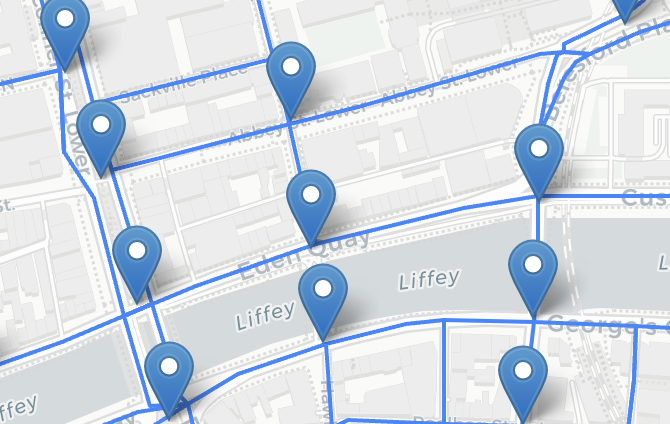
\includegraphics[width=0.5\textwidth]{dataset.png}
  \caption{Snapshot of sensor locations plotted along with road network from Overpass API}
  \label{fig:dataset}
\end{figure}


\subsection{Model Parameters}

For all experiments, we set hyperparameters \(T = 3\), representing the number of consecutive timesteps to consider for prediction and imputation tasks. For all tasks, we optimize the model input by assuming the locality of traffic within such a timespan and that any changes to a particular node are only dependent on nodes "close" to it. During training, we train on subgraphs consisting of node clusters instead of the entire graph at once. Specifically, a subgraph is generated by choosing a node \(u\) at random and then selecting all nodes that are at a distance less than \(\sigma\) to it. Formally, for \(G(V, E)\), the subgraph is defined as \(G_{\text{sub}} = G\{v \in V \mid \text{dist}(u, v) < \sigma\}\). For our experiments, we set \(\sigma\) to \(2.5\ km\), which is reasonable as clusters usually contain 20 to 30 nodes within this range.

After sampling, as stated, we use an 80-20 test-train split, meaning the model is trained on 80\% of the samples, and performance is verified on new unseen data comprising 20\% of the samples. The data is then modified based on the task at hand. For imputation, we followed the MCAR (Missing Completely at Random) distribution and randomly masked values both spatially and temporally, based on a parameter defined as the miss rate. We tested our model on miss rates of 10\%, 20\%, 30\%, and 40\%. For prediction, we use the full data of three timesteps to predict the fourth step by masking the values along the last timestep dimension. For the re-assignment task, i.e., task (iii), we only consider one timestep and re-assign values for that same timestep but with modified spatial geometry.

\subsection{Baselines}

We compare our \name\ model with several existing approaches across different domains, including various mathematical analysis and deep learning techniques that are commonly used for these tasks.

For imputation, one of the simplest approaches is \textit{KNN}. For prediction, \textit{ARIMA} (AutoRegressive Integrated Moving Average) \cite{arima} is employed. Matrix factorization methods such as \textit{TRMF} (Temporal Regularized Matrix Factorization) \cite{trmf} use latent factors for predictions, with \textit{BTRMF} (Bayesian Temporal Regularized Matrix Factorization) extending TRMF within a Bayesian framework. For both TRMF and BTRMF, we use a rank of 10, 1000 burn-in iterations, and 200 Gibbs iterations.

\textit{LRTC-TNN} (Low-Rank Tensor Completion with Truncated Nuclear Norm) \cite{lrtc} is a method for tensor completion, using parameters $\rho = 1e-5$, $\theta = 0.25$, and $\epsilon = 1e-4$. \textit{BGCP} (Bayesian Gaussian Process Factorization) utilizes Bayesian inference. For BGCP, we use similar burn-in and Gibbs iterations and set the rank to 30. It is important to note that these model baselines are applicable only to task (i) and task (ii), and not to task (iii) since they were not designed for that task.

Additionally, we employed deep learning methods. For imputation, we used the \textit{Denoising AutoEncoder} (DAE) \cite{dae} model, which is effective in learning meaningful representations of the data while handling missing values. For prediction tasks, we utilized an \textit{LSTM} (Long Short-Term Memory) \cite{lstm} model, as LSTM networks are well-suited for capturing temporal dependencies in sequential data.


\subsection{Evaluation metrics}

To evaluate the performance of the different methods and compare them, we use RMSE (Root Mean Squared Error) and MAPE (Mean Absolute Percentage Error). These metrics are defined as follows:

\[
\text{RMSE} = \sqrt{\frac{1}{n} \sum_{i=1}^{n} (y_i - \hat{y}_i)^2}
\]

\[
\text{MAPE} = \frac{1}{n} \sum_{i=1}^{n} \left| \frac{y_i - \hat{y}_i}{y_i} \right| \times 100\%
\]

where \( y_i \) represents the true value, \( \hat{y}_i \) represents the predicted value, and \( n \) is the number of samples.